\documentclass{article}

\usepackage[utf8]{inputenc}
\usepackage{graphicx}
\usepackage{imakeidx}
\usepackage{biblatex}
\addbibresource{references.bib}

\begin{document}
\newcommand{\myTitle}{App asistencial para niños prematuros}

\newcommand{\myAuthor}{Cristian Manuel Suárez Vera}

\newcommand{\tutor}{Alexis Quesada Arencibia}

\title{\myTitle}

\begin{titlepage}

\topmargin = 0pt
\headheight = 0pt

\begin{figure}

\includegraphics[width=15cm]{images/logo_eii.jpg}
\end{figure}

\begin{center}

\Large{Grado en Ingeniería Informática}

\vfill
\Large{Trabajo Fin de Grado}

\vfill
\Huge{\textbf{\myTitle}}

\vfill
\Large{\textbf{\myAuthor}}

\vfill
\Large{Tutor: \textbf{\tutor}}

\vfill
\large{Las Palmas de Gran Canaria}

\large{\today}

\end{center}


\end{titlepage}
\makeatother

\tableofcontents
\listoffigures
\listoftables

\newpage

% TODO: agradecimientos

\begin{abstract}
    Premature children present a unique characteristic and that is why
    It needs special care. One of the fields that they require is the physiotherapy,
    which will focus on encouraging, facilitating ..., the different stages of motor
    development. This assistance involves the realization of therapies that
    modification according to their age and their evolution. In addition, parents
    are entrusted continue with the therapy at home, performing the exercises that
    the professional advise This is a challenge of great difficulty for parents
    number of different exercises and postures that they must remember. In this
    project has been developed a multiplatform application prototype to support
    parents and physiotherapists to facilitate the monitoring of therapies
    settled down.\end{abstract}

\begin{abstract}
    Los niños prematuros presentan unas características únicas y es por ello que
    necesitan de unos cuidados especiales. Uno de los ámbitos que requieren es la
    fisioterapia, que irá enfocada a estimular, facilitar…, las diferentes etapas
    del desarrollo motor. Esta asistencia conlleva la realización de terapias que
    varían en función de su edad y su evolución. Además, se encomienda a los padres
    continuar con la terapia en casa, realizando los ejercicios que el profesional
    aconseja. Esto supone un reto de gran dificultad para los padres dada la
    cantidad de ejercicios y posturas diferentes que deben recordar. En este
    proyecto se ha desarrollado un prototipo de app multiplataforma de apoyo a
    padres y fisioterapeutas para facilitar el seguimiento de las terapias
    establecidas.
\end{abstract}
\clearpage

\section{Estado del arte}
%  ESTADO  ACTUAL  Y  OBJETIVOS INICIALES: situación actual del tema relacionado 
%  con el TFT, motivación y objetivos que se pretenden cubrir con este trabajo 
%  (deberán recogerse obligatoriamente los objetivos inicialmente planteados en el TFT-01)
El pasado 7 de abril de 2005 en la 58ª asamblea mundial de la salud la Organización Mundial
de la Salud\cite{OMS} trató el la temática de la cibersalud (conocida también como e-Salud
o e-Health) y su importancia en la actualidad. Indicando que esta "consiste en el apoyo que
la utilización costoeficaz y segura de las tecnologías de la información y las comunicaciones
ofrece a la salud y a los ámbitos relacionados con ella, con inclusión de los servicios de
atención de salud, la vigilancia y la documentación sanitarias, así como la educación, los
conocimientos y las investigaciones en materia de salud"\cite{58-asamblea}.

Dados los avances de las nuevas tecnologías y que estas están presentes en facetas de
nuestra vida diaria como: educación, comunicación, producción industrial. ¿Porqué no
en la medicina? No decimos que estas no existan, porque las hay, aplicaciones como
BilliCam \cite{BilliCam} con la que puedes sacar una foto a tu bebé con una tarjeta de
calibración en el vientre. Con esto la app distingue la luz y el tono de la piel del recién
nacido, y con ello busca el diagnóstico de la ictericia neonatal. Como esta hay otras
aplicaciones las cuales buscan solucionar problemas muy específicos.

Este no es el ámbito que nosotros nos incumbe, lo que buscamos lograr es ayudar, tanto a
los médicos como a pacientes el seguimiento y realización, respectivamente, de ejercicios
para el apoyo del bebé en sus primeros meses. Algo que supondría un cambio a mejor en el
sistema actual de atención fisioterapéutica facilitando a ambas partes.

\bigskip
Actualmente el índice de niños prematuros ha aumentado considerablemente. Estos niños presentan
unas características únicas y es por ello que necesitan de unos cuidados especiales. Uno de los
ámbitos que requieren es la fisioterapia, que irá enfocada a estimular, facilitar, etc. las
diferentes etapas del desarrollo motor, favoreciendo su su desarrollo y previniendo posibles
complicaciones a lo largo de su crecimiento, sobretodo en su primer año de vida.

Para conseguir este fin, el Servicio Canario de Salud dispone de un servicio de fisioterapia
para toda la isla que atiende y realiza un seguimiento de los casos en los que se requiere de
una asistencia profesional.

En general, esta asistencia conlleva la realización de una serie de terapias, consistentes en
la ejecución de una serie de ejercicios con el bebé que varían en función de su edad y su
evolución. Además, se encomienda a los padres continuar con la terapia en casa, realizando
los ejercicios que el profesional aconseja. Esto supone un reto de gran dificultad para los
padres dada la cantidad de ejercicios y posturas diferentes que deben recordar. Esto hace que
los padres busquen comunicarse con los profesionales para que estos comprueben si están
realizando correctamente el ejercicio concreto mediante el envío de vídeos por plataformas
externas. Además, dada la gran demanda del servicio, en ocasiones se ven desbordados y la
frecuencia con la que pueden citar a los bebés es muy inferior a la deseada, no pudiendo
realizar un seguimiento de forma óptima. Por último, dado que el servicio se ofrece para la
atención de niños prematuros de todos los municipios de la isla, el desarrollo de una herramienta
informática de apoyo puede ser de gran utilidad para evitar, en ocasiones, el desplazamiento
de las familias.

\bigskip
\subsection{Objetivos}
Nuestra \textbf{\myTitle} tiene como objetivos básicos:
\begin{enumerate}
    \item Poner a disposición de los padres material gráfico y multimedia de apoyo que permita desarrollar los ejercicios indicados por el fisioterapeuta.
    \item Grabar vídeos e instantáneas a los padres para que puedan registrar la evolución del bebé de forma que dicho material pueda ser supervisado por el fisioterapeuta.
    \item La comunicación Fisioterapeuta – Padres.
    \item Realizar una valoración de la evolución del bebé.
    \item Evaluar la utilidad de los materiales por parte de los padres.
\end{enumerate}

Dado el tiempo del que hemos dispuesto para la realización de la misma, hemos decidido abarcar
dos de los objetivos más relevantes para esta primera fase de la aplicación, los cuales son el
punto número 1 y el número 2. Con los que los padres ya podrán realizar los ejercicios indicados
con mayor seguridad teniendo a su disposición material de apoyo y, por su parte el médico podrá
ver la evolución del bebé para prevenir cualquier otro problema que pueda surgir.

\clearpage

\section{Justificación de las competencias}
%  JUSTIFICAIÓN DE LAS COMPETENCIAS ESPECÍFICAS CUYBIERTAS: indicar, sólo para 
%  las competencias específicas relacionadas de forma más directa con el trabajo 
%  desarrollado, cómo se han cubierto con este TFT.
% COMPETENCIAS: CII08 – CII012 – CII016 – IS01 – IS02 – IS03 – IS04

\subsection{Comunes a la Ingeniería informática}
\subsubsection{CII08}
\textit{"Capacidad para analizar, diseñar, construir y mantener aplicaciones de forma
robusta, segura y eficiente, eligiendo el paradigma y los lenguajes de programación más
adecuados."}

\subsubsection{CII012}
\textit{"Conocimiento y aplicación de las características, funcionalidades y estructura de las
bases de datos, que permitan su adecuado uso, y el diseño y el análisis
e implementación de aplicaciones basadas en ellos."}

\subsubsection{CII016}
\textit{"Conocimiento y aplicación de los principios, metodologías y ciclos de vida de la
ingeniería de software."}

\subsubsection{IS01}
\textit{"Capacidad para desarrollar, mantener y evaluar servicios y sistemas software que
satisfagan todos los requisitos del usuario y se comporten de forma fiable y
eficiente, sean asequibles de desarrollar y mantener y cumplan normas de
calidad, aplicando las teorías, principios, métodos y prácticas de la ingeniería del
software."}

\subsubsection{IS02}
\textit{"Capacidad para valorar las necesidades del cliente y especificar los requisitos
software para satisfacer estas necesidades, reconciliando objetivos en
conflicto mediante la búsqueda de compromisos aceptables dentro de
las limitaciones derivadas del coste, del tiempo, de la existencia de sistemas ya
desarrollados y de las propias organizaciones."}

\subsubsection{IS03}
\textit{"Capacidad de dar solución a problemas de integración en función de las estrategias,
estándares y tecnologías disponibles."}

\subsubsection{IS04}
\textit{"Capacidad de identificar y analizar problemas y diseñar, desarrollar,
implementar, verificar y documentar soluciones software sobre la base de
un conocimiento adecuado de las teorías, modelos y técnicas actuales."}

\clearpage

\section{Aportaciones al entorno}
%  APORTACIONES: justificar que es lo que este TFT aporta a nuestro entorno socio-economico,
%  tecnico o cientifico.
\subsection{Entorno socio-económico}
El desarrollo de este proyecto ofrecerá tanto a padres como doctores un medio de comunicación
y visualización de ejercicios rápido, sencillo y con el que evitar gasto de papel que conlleva
el sistema actual. A día de hoy a los padres se le dan hojas con las ilustraciones referentes
a los ejercicios que tienen que realizar.

\medskip
El gasto masivo de papel es un tema que está a la orden del día, puesto que de él deriva la
tala de árboles, la cual tiene varias consecuencias negativas:
\begin{enumerate}
    \item Cambios de clima debido a la falta de árboles para la retención de humedad, con lo que aumenta la posibilidad de sequías.
    \item Destrucción de ecosistemas y la perdida de biodiversidad que ello conlleva.
    \item Disminución del medio de transformación de dióxido de carbono en oxigeno, aumentando el efecto invernadero y aumentando las enfermedades respiratorias de la población.
\end{enumerate}

\bigskip
Además del reducir el impacto negativo en el medioambiente, reduce gastos en los centros
que hagan uso de la aplicación. Eliminando el gasto referente al papel y reduciendo el
tiempo que los doctores utilizan para solventar dudas del paciente debido a:
\begin{enumerate}
    \item Mayor rapidez en la comunicación doctor-paciente, es instantánea.
    \item Ahorro por parte de los pacientes en cuanto a desplazamiento en combustible y tiempo.
    \item Mayor facilidad para recordar el ejercicio, dado que se provee de material en forma de vídeo (en caso de que se considere necesario).
    \item Seguridad por parte del paciente, al tener material y medio de comunicación directo con su doctor que puede consultar en cualquier momento.
    \item Facilidad para el doctor a la hora de realizar seguimientos.
\end{enumerate}

\medskip
Este proyecto tiene consecuencias positivas tanto en el medio ambiente, como para los doctores
y familias con hijos prematuros.

\subsection{Personal}
A nivel personal, este proyecto resulta enriquecedor. Ha sido desarrollado desde cero
pasando por todas y cada una de las fases de un proyecto informático desde el análisis
hasta la implementación.

\medskip
Gracias a ello se ha podido reforzar los conocimientos adquiridos durante la carrera referentes
a cada una de estas fases de desarrollo, así como a las herramientas y tecnologías utilizadas. A
nivel de implementación la aplicación móvil a servido para conocer nuevas tecnologías como
\textit{Ionic}, \textit{TypeScript}, \textit{SCSS}, \textit{Firebase}.
\clearpage

% TODO: normativa y legislacion

\section{Metodología de trabajo y planificación del proyecto}
\subsection{Metodología de trabajo}
Inicialmente se planteó una metodología de trabajo inspirada en el modelo de ciclo de vida del software
basado en prototipos. Siendo el prototipo una aplicación con al menos una funcionalidad implementada,
que se le presentará al cliente con la que podrá ver los avances y como se resuelve el requisito planteado.
Además este podrá dar su opinión al respecto permitiendo modificar la forma en la que se implementa si no
es lo esperado o no se ajusta con lo que había previsto, con ello se esperaba obtener un software a
medida que se ajustara de la mejor forma posible a las problemáticas.

\medskip
Una vez realizada la primera reunión con el cliente y planteada la metodología prevista este lo consideró
inviable, puesto que no tiene la disponibilidad necesaria para hacer reuniones con frecuencia y probar el
resultado obtenido hasta ese momento. Por ello hubo que cambiar la metodología a una clásica en cascada,
esta consiste en plantear las tareas de manera secuencial e ir solucionando cada una solamente después de
haber terminado la anterior. Una vez se ha concluido con todas, ya tendremos nuestro proyecto finalizado
y listo para presentar y validar.

\medskip
Se ha decidido utilizar finalmente esta metodología al ser la que mejor se ajusta a las necesidades del
cliente y por la fuerte dependencia entre las funcionalidades. Puesto que la mayoría necesitan de que
exista previamente otra.

\subsection{Planificación inicial del proyecto}
Tras un estudio del estado del arte actual, se decidió en la primera fase del proyecto hacer un análisis
de la problemática con el que decidir cuales son los actores que intervienen en el sistema, es decir,
cuales serán los usuarios que interactuarán con él y que funcionalidades podrán usar cada uno. Estas
funcionalidades también se decidirán en esta primera fase de análisis. Para todo ello se hará uso de
de los diagramas de casos de uso \cite{casos-de-uso} y las tablas de especificación de los casos de
uso \cite{tabla-especificacion-casos-de-uso}.

\medskip
Una vez se decidió los actores que actúan en el sistema y los requisitos (funcionalidades) de cada uno
se continuó con un prototipo de la interfaz, para poder tener una primera visualización de los objetivos
que se tenía con esta aplicación.

\medskip
Este prototipo fue de gran ayuda puesto que se solucionaron dudas que había en ese momento sobre
las funcionalidades planteadas y las soluciones propuestas, además planteó otras dudas sobre otros requisitos
que no se habían planteado en un primer momento. A continuación se comentarán el cambio más significativo.

\medskip
Inicialmente en la primera pantalla de los pacientes, se usó una lista con una imagen del ejercicio y el
título de este como se puede ver en la figura \ref{patient-home-v1}. Tras la presentación de este primer prototipo,
se decidió que estas ocupaban demasiado espacio en la pantalla y eran molestas. Es por ello que se pasó a mostrar los
ejercicios solamente con el título.

\begin{figure}[!h]
    \centering
    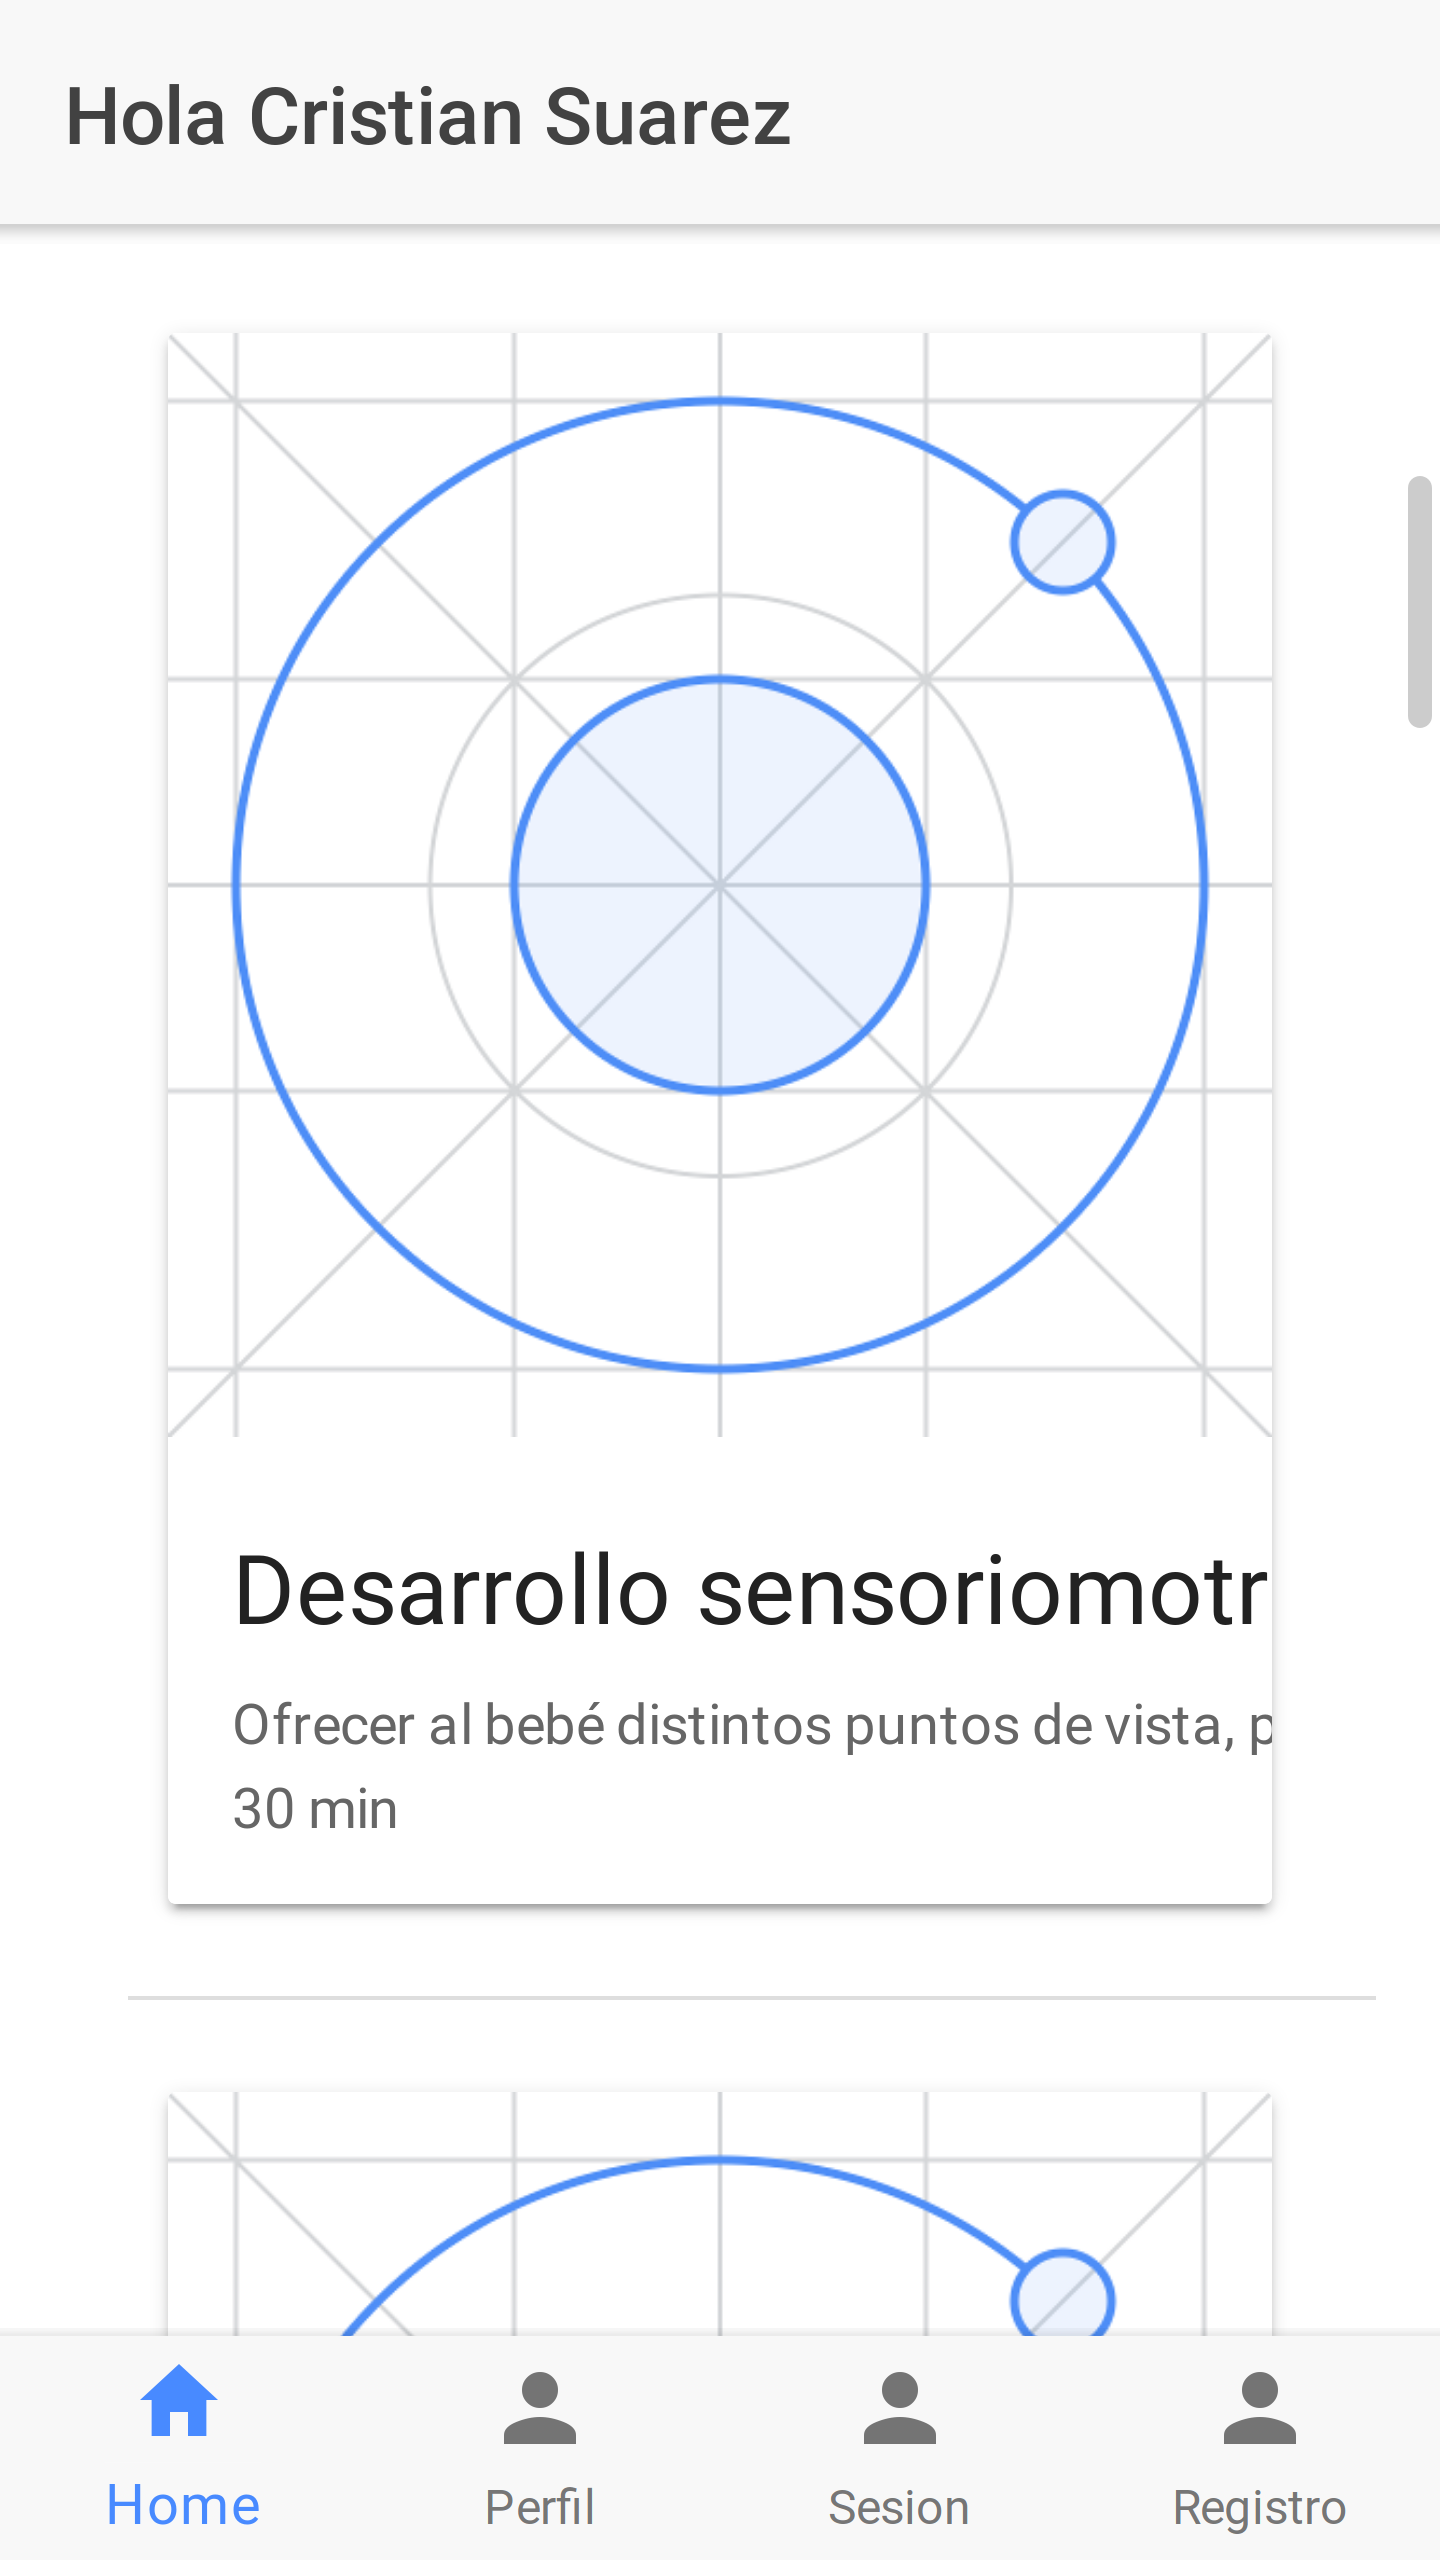
\includegraphics[width=0.5\textwidth]{images/screenshots/patient-home-v1.png}
    \caption{Pantalla inicial paciente, prototipo}
    \label{patient-home-v1}
\end{figure}


\medskip
Con esa parte ya solventada se empezó con el aprendizaje de la tecnología a usar, \textit{Ionic} \cite{ionic}.
Para el aprendizaje de este \textit{framework} se hizo una pequeña aplicación de gestión de tareas
sugerida en el propio libro de aprendizaje utilizado, \textit{"Learning ionic : buid hybrid mobile
applications with HTML5"} \cite{ionic-book}. Para complementar el aprendizaje de este libro se realizó
varios tutoriales \textit{online}, con todo ellos se adquirió experiencia y fluidez en el uso del
\textit{framework}.

\medskip
Una vez acabada la fase de aprendizaje se continuó con el desarrollo, este contemplaba las funcionalidades
que se describirán a continuación:

\medskip
\textbf{Las comunes para todos los usuarios:}
\begin{enumerate}
    \item Registro e inicio de sesión
    \item Vista del perfil personal
    \item Editar el perfil
    \item Enviar y reproducir vídeos
    \item Ver ejercicios
\end{enumerate}

\medskip
\textbf{Específicas del paciente:}
\begin{enumerate}
    \item Marcar ejercicio como hecho
\end{enumerate}

\medskip
\textbf{Específicas del doctor:}
\begin{enumerate}
    \item Buscar paciente
    \item Asignar ejercicio
    \item Añadir observaciones al ejercicio que se va a asignar
    \item Ver el perfil de un paciente
    \item Ver la evolución de un paciente
\end{enumerate}

\subsection{Ajustes en la planificación del proyecto}
La tarea de implementación (\textbf{Tarea 2.4}) se tuvo que retrasar según lo previsto inicialmente,
puesto que la tarea de aprendizaje (\textbf{Tarea 2.3}) del \textit{framework} llevó más de lo esperado.
A ello hay que añadirle que se decidió incorporar una funcionalidad que no se esperaba realizar,
la referente con la creación de un chat paciente - doctor y todo lo que ella conlleva, porque se
consideró que esta sería la forma más intuitiva para el usuario de enviar vídeos. Esto hizo que además
de retrasarse la implementación aumentase el tiempo que requiere. Es por todo ello que
dentro de la fase de diseño e implementación la distribución de tiempo entre tareas no fue el esperado.
Y finalmente la última funcionalidad referente al envío de vídeos no se pudo completar al cien por cien.

\medskip
En el siguiente cuadro \ref{planificacion-inicial} se muestran los casos de uso anteriores con una breve descripción.
\begin{table}
    \begin{tabular}{|lp{12cm}|}
        \hline
        FASES (HORAS) & TAREAS \\ \hline

        \multirow{3}{*}{Análisis}
        \multirow{3}{*}{(70)}
        & Tarea 1.1: Estudio del problema y soluciones actuales \\
        & Tarea 1.2: Captura de los requisitos del sistema \\
        & Tarea 1.3: Prototipo de la interfaz de usuario del sistema \\ \hline

        \multirow{4}{*}{Diseño}
        \multirow{4}{*}{(160)}
        & Tarea 2.1: Diseño de la estructura del sistema \\
        & Tarea 2.2: Diseño de la base de datos \\
        & Tarea 2.3: Aprendizaje de tecnologías de implementación: Ionic 2, etc \\
        & Tarea 2.4: Implementación de prototipos de la aplicación móvil \\ \hline

        \multirow{2}{*}{Pruebas}
        \multirow{2}{*}{(30)}
        & Tarea 3.1: Pruebas de funcionamiento de la aplicación móvil \\
        & Tarea 3.2: Pruebas de integración y rendimiento de la aplicación móvil \\ \hline

        \multirow{2}{*}{Documentación}
        \multirow{2}{*}{(40)}
        & Tarea 4.1: Realización de la memoria \\
        & Tarea 4.2: Realización de la presentación del TGF \\ \hline
    \end{tabular}

    \caption{Tabla planificación inicial del proyecto.}\label{planificacion-inicial}
\end{table}
\clearpage

\section{Tecnologías y herramientas utilizadas}
\subsection{Tecnologías}
\begin{itemize}
    \item\textbf{Ionic:} \textit{framework} de desarrollo para aplicaciones móviles, este es
    de código abierto. Está basado en varias tecnologías entre ellas HTML, Typescrip, SCCS. La
    ventaja de este \textit{framework} para el desarrollo multiplataforma es el tener que
    desarrollar solamente una versión de la aplicación y luego esta se puede exportar a IOS,
    Android o Windows Phone.
    \item\textbf{Ionic View App:} aplicación móvil con la que poder visualizar el proyecto que
    estás desarrollando, para poder hacer uso de ella tienes que subir a la web de ionic tu
    proyecto, una vez ahí te dan un código único identificador que introduces en tu teléfono
    tras esto te cargará la aplicación como si la tuvieses instalada y podrás probarla de manera
    nativa.
    \item\textbf{Angular:} \textit{framework} de \textit{JavaScript} de código abierto mantenido
    por Google usado principalmente para la creación de \textit{SPA}\cite{SPA} de manera más fácil
    a las existentes en la actualidad, además este te permite una creación de pruebas de forma más
    sencilla.
    \item\textbf{Cordova:} entorno de desarrollo para aplicaciones móviles el cual está basado en
    HTML, JavaScript y CSS, facilita el empaquetado de todo esto dependiendo del dispositivo y
    hace que no tengas que conocer la \textit{API}\cite{api} de cada plataforma por separado y
    hacer un tratamiento individual para cada una de ellas.
    \item\textbf{Typescript:} lenguaje de programación basado en JavaScript el cual mejora las
    desventajas o problemas que pudiera tener JavaScrip añadiendo un tipado estático y clases,
    entre otras mejoras. Esto hace que su uso sea más cómodo y al estar basado en JavaScript si
    hiciera falta escribir partes de código en JavaScrip puro se puede hacer sin problemas.
    %    \item\textbf{JavaScript:}
    \item\textbf{HTML5:} lenguaje básico de elaboración de páginas web. Es un estándar con el que
    estructurar las distintas páginas/ventanas de nuestra aplicación. Este se considera el lenguaje
    más importante para el crecimiento de la \textit{World Wide Web} (WWW), y ha sido adoptado por
    todos los navegadores actuales para la visualización de páginas webs.
    \item\textbf{SCSS:} \textit{Sassy CSS} al igual que con \textit{TypeScrip} es una ampliación del
    CSS clásico con mejoras tales como la creación de variables de manera más cómoda e intuitiva.
    Al ser una ampliación de CSS se puede escribir CSS clásico en él y lo interpreta correctamente.
    \item\textbf{Firebase:} plataforma con múltiples funcionalidades para la creación de aplicaciones
    móviles, en ella podemos encontrar sistemas de autenticación, base de datos, almacenamiento de
    datos, etc. Se ha decidido usar esta por su fácil uso y gran cantidad de documentación de calidad
    de la que dispone.
    \item\textbf{Git:} sistema de control de versiones con el que gestionar la evolución de la
    aplicación guardando los estados de todos los ficheros por los que va pasando durante el
    desarrollo, de esta manera si hubiese algún problema se puede deshacer los cambios hasta ese
    punto.
\end{itemize}

\subsection{Herramientas}
\begin{itemize}
    %    \item\textbf{Firefox:} explorador web en el que previsualizar la aplicación durante el desarrollo
    \item\textbf{WebStorm:} IDE para trabajar con tecnolgías web, desarrollado por la empresa
    \textit{JetBrains}\cite{jetbrains}. Cuenta con editores para HTML, JavaScript, PHP,
    Typescript, SCSS entre otros además de autocompletado, funciones de refactorización
    automática y depurador.
    \item\textbf{StarUML:} programa de creación de diagramas, soporta distintos tipos de estos
    diagramas de clases, diagramas de casos de uso, etc.
    \item\textbf{Github:} portal web el cual soporta el sistema de control de versiones de git,
    donde poder subir tu proyecto gestionado con git y ver de manera visual todo lo que ello conlleva
    además el proyecto puede ser público, si se quiere, pudiendo cualquier persona que lo vea
    sugerir mejoras a este o posibles cambios.
\end{itemize}

\subsection{Servidores}
\begin{itemize}
    \item\textbf{Firebase, base de datos en tiempo real:} para el guardado de datos se ha usado
    una base de datos no relacional que provee \textit{firebase} por las ventajas que esta proporciona
    frente a una relacional. La principal por la que esta se tuvo en cuenta ha sido que permite
    datos sean variables, puedan cambiar a lo largo del tiempo sin tener que para la base de datos
    debido a que aún el cliente no tiene claro como quiere guardar los ejercicios, además estas
    bases de datos permiten mayor accesibilidad al consumir menos recursos para su mantenimiento.
\end{itemize}

\clearpage

\section{Análisis}
\subsection{Actores}
Se han identificado dos actores principales los cuales se expondrán a continuación.

\subsubsection{Doctor}
Personal del centro médico el cual tendrá pacientes a su cargo, sus funciones serán
las siguientes:
\begin{itemize}
    \item Buscar pacientes entre los registrados en el sistema.
    \item Asignar ejercicios a un paciente.
    \item Añadir observaciones a los ejercicios que se van a asignar.
    \item Ver perfil de un paciente.
    \item Ver evolución de un paciente.
\end{itemize}

Toda funcionalidad tienen como objetivo que el doctor pueda indicarle a sus
pacientes los ejercicios que este tiene que realizar y si en su caso concreto tendrá
que tener en cuenta alguna variación del original dejarlo indicado en las observaciones.
Además tendrá que poder ver el perfil del paciente para poder consultar sus datos, en caso
de que le fueran necesarios.

\subsubsection{Paciente}
Otro actor que se ha identificado es el paciente con la siguiente funcionalidad:
\begin{itemize}
    \item Ver ejercicio.
    \item Marcar ejercicio como hecho.
\end{itemize}

Con esta funcionalidad se busca que el paciente pueda llevar un control de los ejercicios
que ha realizado y esto pueda ser consultado por el doctor en cualquier momento.

\medskip
Además estos actores principales tendrán funcionalidades \textbf{comunes:}

\begin{itemize}
    \item Registro en la aplicación.
    \item Inicio de sesión.
    \item Ver perfil.
    \item Editar perfil.
    \item Iniciar chat.
    \item Enviar y visualizar vídeos por el chat.
\end{itemize}

Estas funciones son necesarias que estén disponibles en ambos actores. Debido a que el chat
es tanto doctor con paciente, como a la inversa. Además, los usuarios tienen que poder
darse de alta en el sistema.
\clearpage

% TODO: diseño

\section{Desarrollo}
\subsection{Ionic}
Se expondrá a continuación las razones por las que se
ha decidido usar ionic como framework de desarrollo para
este proyecto:

\begin{itemize}
    \item El código se escribe una vez y se usa en todas
    las plataformas, con ionic solo se tiene que escribir
    una vez la lógica que va a seguir y esta puede ser
    compilada luego en la plataforma que se requiera.
    \item Los componentes por defecto que trae para el
    desarrollo de la interfaz dan un buen acabado, sin
    tener que modificar la mayoría de ellos. Lo que permite
    ahorrar tiempo en este apartado.
    \item Se puede comprobar el comportamiento de manera rápida
    y fácil ya que permite ejecutar la aplicación en un
    explorador como si se tratase de un dispositivo móvil.
    Además incluye un apartado donde se puede ver las tres
    versiones de compilación y comprobar el comportamiento
    en cada una de ellas por separado sin tener un dispositivo
    donde instalar la aplicación.
    \item Gran cantidad de documentación oficial y no oficial
    así como tutoriales escritos como en vídeo, de buena calidad.
    \item Lo apoya una gran comunidad y de calidad, lo que hace
    junto al punto anterior que la búsqueda de una solución a
    problemas que puedan surgir sea rápida y eficaz.
    \item Trabaja con tecnologías modernas, con lo que
    su arquitectura es limpia y robusta.
    \item Al estar basado en lenguajes básicos y estandarizados
    hace que su uso resulte en ciertos puntos intuitivo.
    \item Lleva varios años en el mercado funcionando y tiene
    cientos de aplicaciones hechas con él, por lo que no es un
    producto tan nuevo como para que pueda tener grandes fallos.
\end{itemize}

\subsection{Estructura del proyecto}

Uno de los puntos buenos que tiene este \textit{framework} es
poseer una estructura de directorios bien conocida y definida,
por ello será fácil navegar por ella incluso para nuevos
desarrolladores que se incorporasen al proyecto.

\medskip
Los principales directorios son los siguientes:

\begin{itemize}
    \item /src/app/: ficheros de configuración de la aplicación.
    \item /src/assets/: ficheros multimedia y recursos estáticos.
    \item /src/enviroments/: ficheros de configuración para los
    distintos entornos (desarrollo o producción)
    \item /src/pages/: directorio donde van ubicados los directorios
    de cada pandalla o componente de la aplicación.
    \item /src/pages/page1/: ficheros referentes a una pantalla en
    concreto en el van el HTML, TS, SCSS (si fuese necesario)
    \item /src/providers/: ficheros de acceso a los datos.
    \item /src/theme/: fichero de estilo genérico en el cual
    se basa la aplicación.
\end{itemize}

% hablar de los distintos tipos de ficheros que hay en el poryecto
% meter trozos de codigo explicando como va el sistema
% y hacer tiempo para hacer un par de paginas mas
% contar la importacia de los buenos nombres
\clearpage

\section{Conclusiones y trabajos futuros}
\subsection{Conclusiones}

En términos generales los objetivos con los que se inició el proyecto han
sido cumplidos, logrando una primera aproximación funcional para
la problemática planteada. Teniendo en cuenta el poco margen de tiempo del
que se dispone en este tipo de proyectos, se ha logrado una buena primera
versión que esperamos que pueda seguir evolucionando y mejorando con el tiempo.

\medskip
La participación y realización de este proyecto ha resultado una
experiencia enriquecedora y formativa. Se ha podido reforzar los
conocimientos adquiridos en la carrera tanto genéricos como específicos
de la Ingeniería del Software. Además de obtener nuevos referentes a
las tecnologías que se han decidido usar como Ionic, TypeScript, Firebase,
entre otras.

\medskip
Al tratarse de un proyecto que se ha iniciado desde cero hasta el final
del mismo ha sido una experiencia nueva, al no haber hecho antes
tal proceso al completo. Si es cierto que se conocían todas sus
fases por separado, pero el poder aplicarlas juntas ha resultado
una experiencia muy positiva.

\medskip
Además, haber buscado una solución a un problema
existente y haber sido capaz de aprender una tecnología nueva,
me ha hecho ver que estos años de universidad
no solamente se han adquirido conocimientos técnicos. También ha
hecho que adquiera una forma de pensar con la que poder buscar soluciones a
problemas y una mentalidad abierta para aprender nuevas cosas
ya sean tecnologías o metodologías de forma más o menos rápida y
fácil.

\medskip
En términos generales este proyecto ha sido una experiencia
muy gratificante. A pesar de sus cambios en medio del desarrollo,
sus horas de aprendiendizaje de nuevas herramienta en las que parecía que
no se avanzaba con el proyecto, las entrevistas
con el cliente y con todo lo ocurrido se puede decir que ha sido
una muy buena experiencia y se ha logrado obtener un resultado cercano al
esperado.

\subsection{Mejoras futuras}
A continuación se describirán mejoras a la funcionalidad
implementada y nuevas funcionalidades que se podrían incorporar, de
cara a completar este proyecto.
\begin{itemize}
    \item Enviar vídeos por el chat, funcionalidad que se tuvo que
    dejar por falta de tiempo y es necesaria para el producto
    mínimo viable.
    \item Permitir usuarios de tipo administrador, el cual pueda añadir
    ejercicios a la base de datos, modificar o eliminar los mismos.
    \item Añadir evaluación de la evolución del paciente, a día de hoy
    solo se puede ver cuando ha realizado el ejercicio.
    \item Enviar esta evaluación por el chat al paciente para que sea
    notificado.
    \item Permitir marcar ejercicio como hecho sin tener que entrar
    en la vista del ejercicio.
    \item Implementar un sistema de notificaciones si un ejercicio
    se ha marcado con una periodicidad diaria y hace más de 20 horas
    que no se ha indicado que se ha realizado.
    \item En el momento del registro permitir más localidades de
    nacimiento, no solamente municipios de Gran Canaria.
    \item Añadir un servicio de gestión de citas, donde el médico
    pueda indicar que tiene una cita con un paciente y este pueda
    ver en su teléfono cuando será la siguiente cita.
    \item Poder notificar tanto paciente como doctor que no podrá
    asistir a la cita.
    \item Notificación cuando la fecha de la cita prevista se acerca.
    \item Clasificar ejercicios por categorías, para ayudar a la búsqueda
    una vez se tenga una gran cantidad de ellos.
    \item Mejorar la estética de la interfaz de usuario, como puede ser,
    añadir un logotipo de la aplicación.
\end{itemize}
\clearpage

\printbibliography
%bibliografía y fuentes de información utilizadas. En el documento debe  indicarse  la  procedencia
%de  las  figuras  y,  en  caso  de  que  se  incluya  texto  literal,  entrecomillarlo

% TODO: anexo 1, manual de usuario
% TODO: anexo 2, manual de instalacion

\end{document}